\documentclass[11pt, reqno]{article}    % use "amsart" instead of "article" for AMSLaTeX format
\usepackage{my_packages}
\usepackage{tikz_packages}
\usepackage[american,siunitx]{circuitikz}
\usepackage{pgfplots}
\pgfplotsset{compat=1.14}
\usepackage[explicit]{titlesec}

% change the formatting for a section (which we're treating as a problem)
\titleformat{\section}[runin]{\normalfont\bfseries}{}{0em}{#1\ \thesection}
\crefformat{section}{problem #2#1#3}
\Crefformat{section}{Problem #2#1#3}

\title{MAE 3134: Final Exam}
\author{Shankar Kulumani}
\date{11 May 2017}                          % Activate to display a given date or no date

\begin{document}
{\noindent\Large \textbf{MAE 3134: Final Exam}}

\section{Problem}\label{prob:bode_response_analysis}

The frequency response of two systems are shown in~\cref{fig:prob1_bode}.
Using the plots, circle the correct descriptions:
\begin{figure}[htbp]
    \centering
    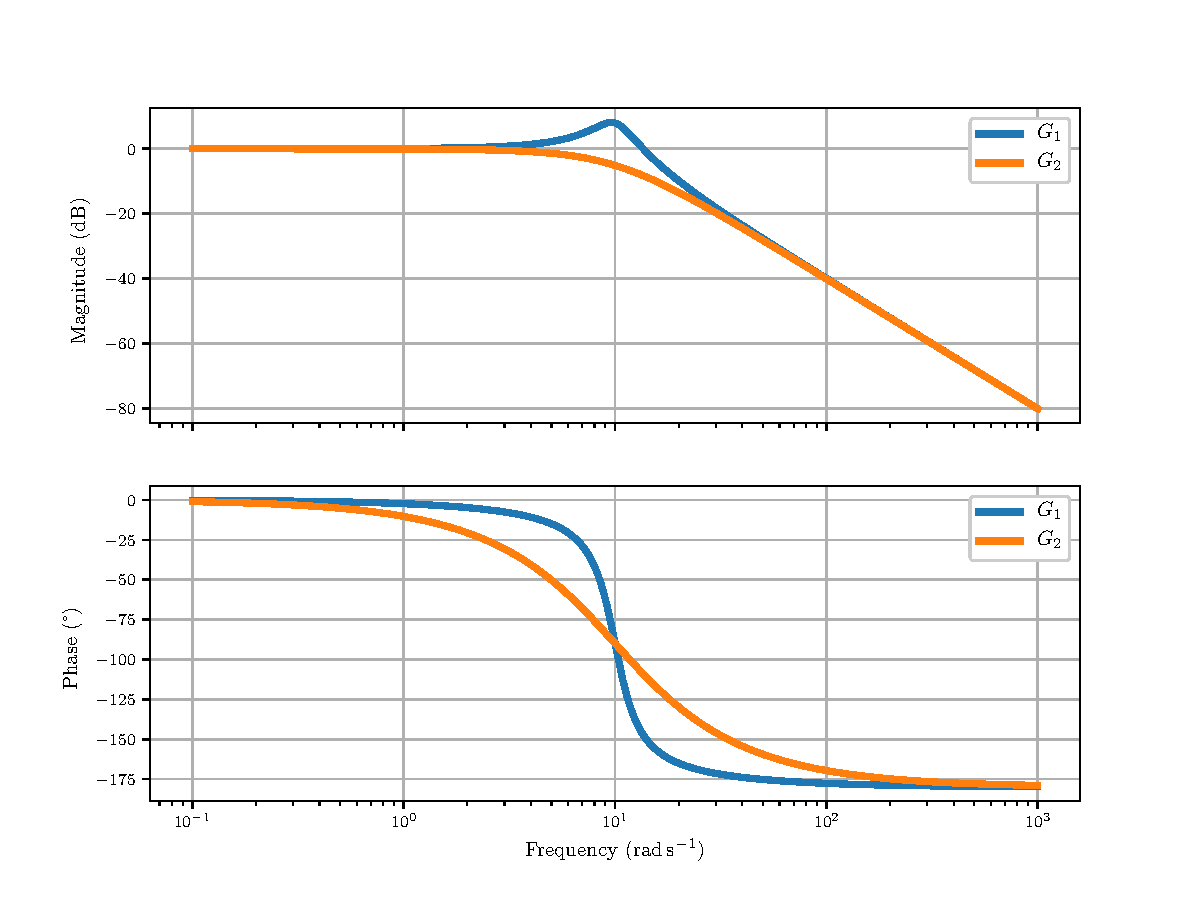
\includegraphics[width=\textwidth, height=0.6\textheight, keepaspectratio]{figures/prob1_bode.pdf}
    \caption{Frequency Response~\label{fig:prob1_bode}}
\end{figure}  

\begin{enumerate}
    \item Which of the following statements are true about the damping ratios of the two systems?
    \begin{enumerate}
        \item The damping coefficients are the same.
        \item The damping coefficient of \(G_1\) is greater than the damping coefficient of \(G_2\).
        \item The damping coefficient of \(G_2\) is greater than the damping coefficient of \(G_1\).
        \item Not enough information to make any statements about the damping ratio.
    \end{enumerate} 
    \item Which of the following statements are true about the general form of \(G_1\)?
    \begin{enumerate}
        \item It is a first order system.
        \item It must have two free \(s\) terms in the denominator since the phase ends at \SI{180}{\degree}.
        \item It must have two free \(s\) terms in the numerator since the final magnitude slope is \SI{40}{\decibel} per decade.
        \item None of the above.
    \end{enumerate}
\end{enumerate}
\clearpage
\section{Problem}\label{prob:sys_response_to_poles}
Elon Musk, CEO of SpaceX and Tesla Motors, has a background in physics but unfortunately has never passed a Linear Dynamics course. 
His newest space vehicle must satisfy the following second order time response specifications for a unit step input:
\begin{itemize}
    \item Percent Overshoot must be less than \(5 \%\),
    \item Rise time less than \SI{1}{\second},
    \item Settling Time less than \SI{5}{\second}.
\end{itemize}
Elon needs your help to choose a set of poles which will satisfy the specifications and save humanity from impending disaster.
\begin{enumerate}
    \item On the s-plane, or complex plane, map out the acceptable regions where you could locate poles and meet the requirements. 
    \item Label the specifications lines and show your work.
    \item Choose a set of poles that will meet the requirements.
\end{enumerate}

\begin{figure*}[htbp]
\centering
\begin{scaletikzpicturetowidth}{0.8\textwidth}
    \begin{tikzpicture}[scale=\tikzscale]
        \draw[help lines, color=gray!30, dashed] (-8, -5) grid (8, 5);
        \draw[->, ultra thick] (-8, 0)--(8, 0) node[right]{Real};
        \draw[->, ultra thick] (0, -5)--(0, 5) node[above]{Imag};
    \end{tikzpicture}
\end{scaletikzpicturetowidth}
\end{figure*}

\clearpage
\section{Problem}

List at least two advantages of state-space or ``modern control'' techniques as compared to ``classical control'' approaches.
\vspace{5cm}
\clearpage
\section{Problem}

The transfer functions of three systems are given as follows:
\begin{align}
    G_1 = \frac{1}{s^2 + 0.2 s+ 1}, \qquad G_2 = \frac{2s +4}{s^2 + 0.5 s + 4}, \qquad G_3 = \frac{-2s + 4}{s^2 + 0.5 s +4}.
\end{align}

\begin{figure}[htbp]
    \centering
    \begin{subfigure}[htbp]{0.4\textwidth} 
        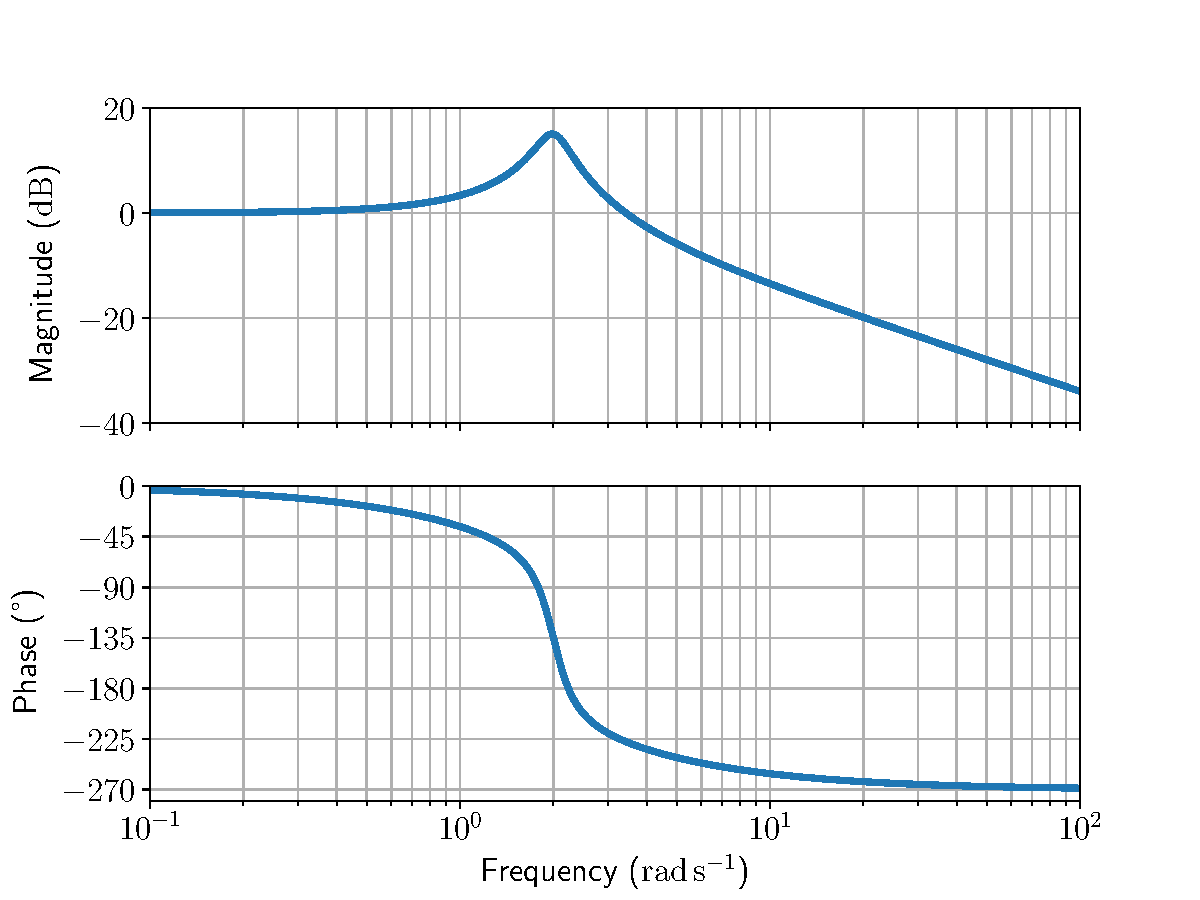
\includegraphics[width=\textwidth]{figures/G3.pdf} 
    \end{subfigure}\\
    \begin{subfigure}[htbp]{0.4\textwidth} 
        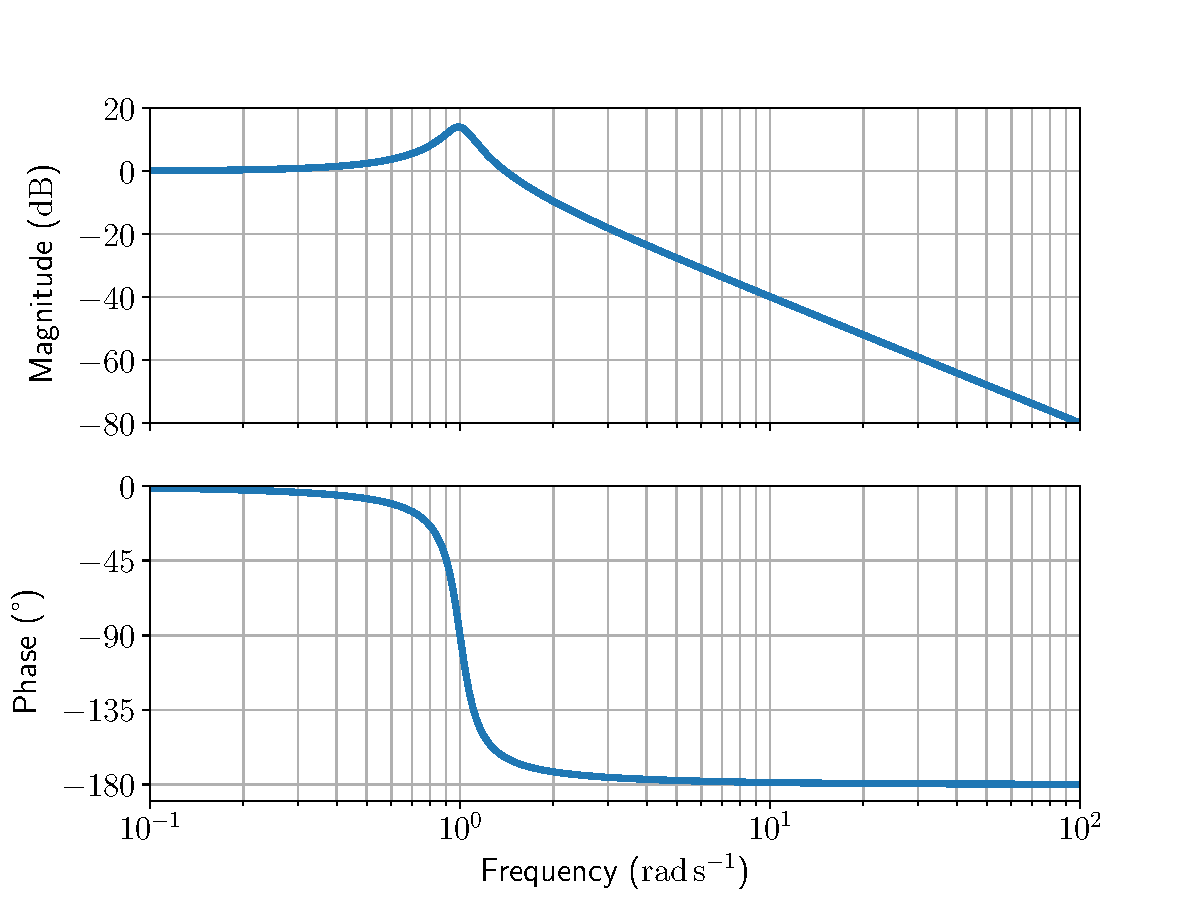
\includegraphics[width=\textwidth]{figures/G1.pdf} 
    \end{subfigure} \\
    \begin{subfigure}[htbp]{0.4\textwidth} 
        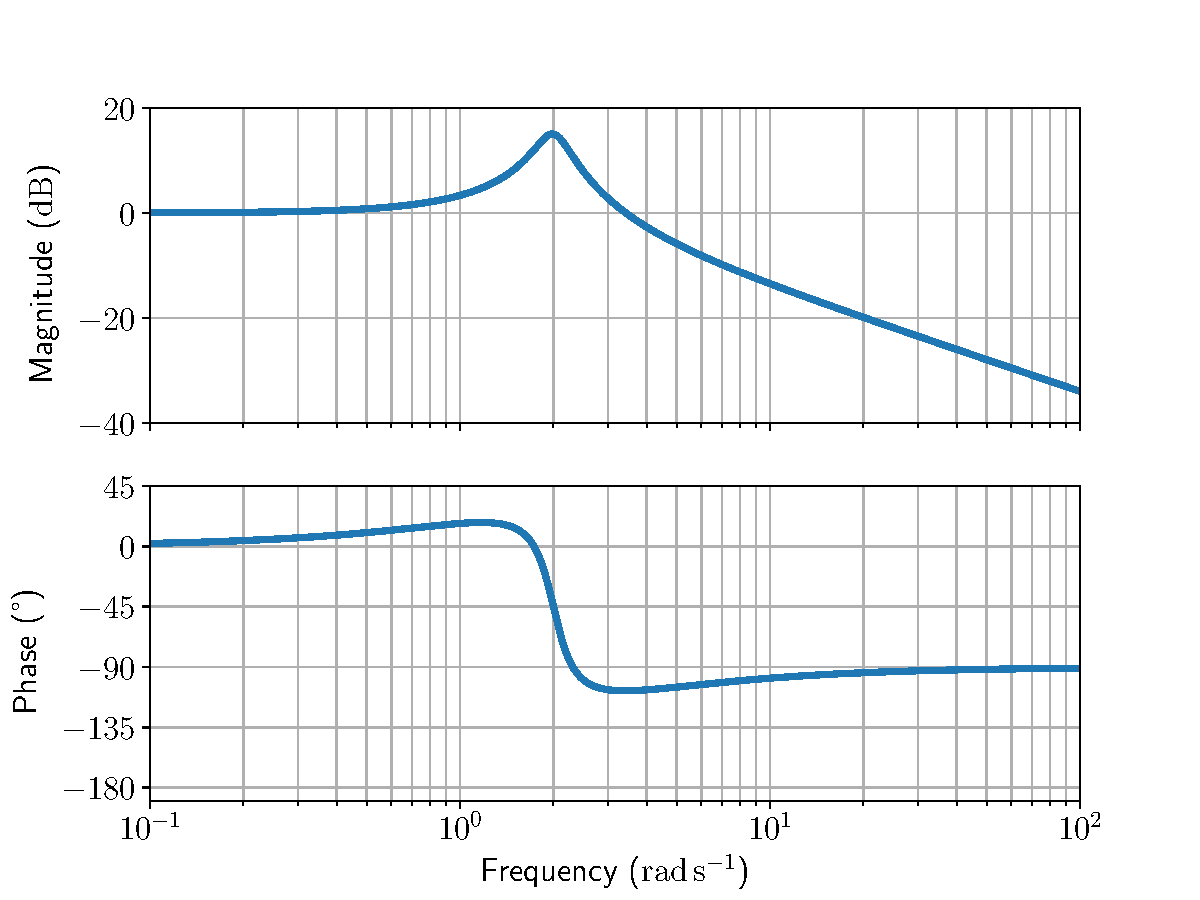
\includegraphics[width=\textwidth]{figures/G2.pdf} 
    \end{subfigure} 
\caption{Bode Plots}
\end{figure}
\end{document}  
